\documentclass[
	fontsize=12pt,
	paper=a4,
	twoside=false,
	numbers=noenddot,
	plainheadsepline,
	toc=listof,
	toc=bibliography
]{scrartcl}

\usepackage[english]{babel} 

%\usepackage[round]{natbib}

\usepackage{amssymb,amsmath}

\usepackage{placeins}
\usepackage{float}

\usepackage{graphicx}
\restylefloat{figure}
\usepackage{subfigure} 

\usepackage{hyperref}

\setlength{\parindent}{0pt}

\title{Alignment of the frames}


\begin{document}

\maketitle

% -----------------------------------------------------------------------------------------------
\section{Channel $01$}
% -----------------------------------------------------------------------------------------------

\begin{figure} [htb]
	\centering
	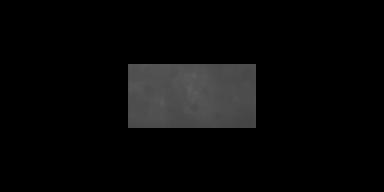
\includegraphics[scale = 0.6]{unaligned_avg_image_channel01.jpg}
	\caption{ Channel $01$: Average image without alignment}
\end{figure}

\begin{figure} [htb] \centering
	\includegraphics[scale = 0.6]{image_alignment_code/aligned_img_channel01.jpg}
	\caption{ Channel $01$: Average image aligned with code by Kamarainen \cite{Kamarainen} }
\end{figure}

\begin{figure} [htb] \centering
	\includegraphics[scale = 0.6]{results_normxcorr/channel01/aligned_avg_image.jpg}
	\caption{ Channel $01$: Average image aligned using cross-correlation}	
\end{figure}

\FloatBarrier

% -----------------------------------------------------------------------------------------------
\newpage
\section{Channel $02$}
% -----------------------------------------------------------------------------------------------

\begin{figure} [htb] \centering
	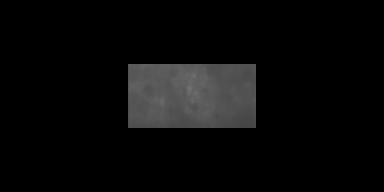
\includegraphics[scale = 0.6]{unaligned_avg_image_channel02.jpg}
	\caption{Channel $02$: Average image without alignment}
\end{figure}

\begin{figure} [htb] \centering
	\includegraphics[scale = 0.6]{image_alignment_code/aligned_img_channel02.jpg}
	\caption{Channel $02$: Average image aligned with code by Kamarainen \cite{Kamarainen} }
\end{figure}

\begin{figure} [htb] \centering
	\includegraphics[scale = 0.6]{results_normxcorr/channel02/aligned_avg_image.jpg}
	\caption{Channel $02$: Average image aligned using cross-correlation}		
\end{figure}



\FloatBarrier

\begin{thebibliography}{1}

\bibitem{Kamarainen}
\url{https://bitbucket.org/kamarain/image_alignment-code/wiki/Home}


\end{thebibliography}


\end{document}